\RequirePackage{plautopatch}
\RequirePackage[l2tabu, orthodox]{nag}

\documentclass[dvipdfmx]{jlreq}
\usepackage{graphicx}
\usepackage{bxtexlogo}
\usepackage{float}
\usepackage{url}

\title{オブジェクト指向プログラミングレポート課題}

\author{5422007 千本木悠  5422009 本江拓海  5422020 池田悠星\\日本大学文理学部情報科学科}
\date{\today}

\begin{document}
\maketitle

\section{システムの概要}
プレイヤーを青四角,敵を赤四角で表す.敵はザコと名付けられた弱い敵と,ボスと名付けられた強い敵とで大きさを変更した.HPバーは緑で表示している.弾幕はそれぞれのキャラクターの色で表示される.プレイヤーの残機は右下に表示される.プレイヤーから発射される銃弾はキーボードのZを押すことで発射される.プレイヤーはマウスで動かすことが可能である.敵に銃弾が当たると敵のHPバーが減少する.HPバーが0になると敵は消滅する.敵の球がプレイヤーに当たるとプレイヤーの残機が減少する.敵のzakoは一定時間で別の場所に動く.

以下の図\ref{fig:screen}は実行画面の概略である.
図中の\textcircled{\scriptsize 1}はプレイヤー,\textcircled{\scriptsize 2}はボス,\textcircled{\scriptsize 3}はザコを表す.いずれも,\ref{sec:class}章に示すCharacterクラスを継承したPlayerクラス,Bossクラス,およびZakoクラスにより実装されている.

\textcircled{\scriptsize 4}はプレイヤーおよび敵の弾幕を表す.誰が射出した弾幕かに関係なく,\ref{sec:class}章に示すGameObjectクラスを継承したBulletクラスにより定義されており,コンストラクタに色や攻撃対象を与えることで機能を区別している.

\textcircled{\scriptsize 5}および\textcircled{\scriptsize 6}はボスおよびザコのHPバーを表す.\ref{sec:class}章に示すGameObjectクラスを継承したHPBarクラスにより定義されている.

\textcircled{\scriptsize 7}はゲーム状況を示す各種テキストを表す.\ref{sec:class}章に示すGameObjectクラスを継承したTextLabelクラスにより定義されている.
なお,Remainingsはプレイヤーの残機を表す.

\begin{figure}[H]
  \centering
  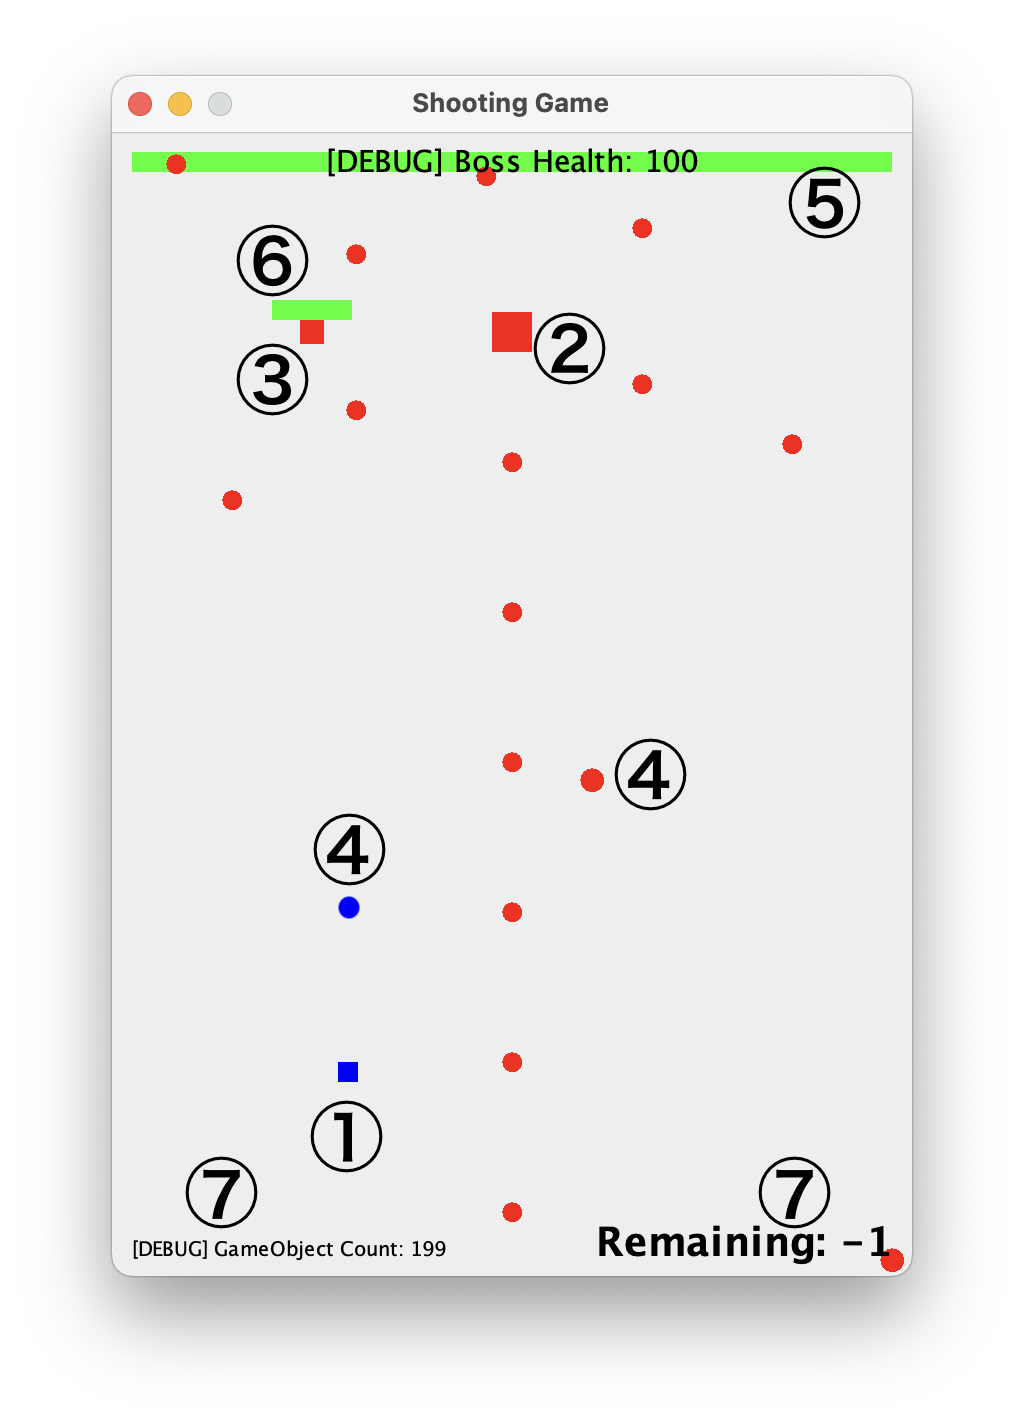
\includegraphics[width=70mm]{figures/screen.png}
  \caption{画面の説明}
  \label{fig:screen}
\end{figure}

\section{クラス設計の指針}
GameObjectクラスですべてのオブジェクト(ゲーム中に登場するキャラクター,UI,弾幕など)を管理することにし,Character,HPBar,Bullet,TextLabelの4つに分けた.

CharacterクラスはEnemy,Playerの2つに分けた.EnemyクラスはZako,Bossといった2つに分けクラス設計を行った.

\section{クラス設計の詳細}\label{sec:class}
図\ref{fig:model}は変更後のクラス設計図である.

Mainクラスでは,すべてのGameObjectの管理をおこなっている.すなわち,あるオブジェクトとあるオブジェクトが衝突したら必要に応じてダメージ処理を与えたり,状況に応じてテキストの内容を変更したりしている.
また,後述する各GameObjectクラスのtask()メソッドを呼び出し,各GameObjectの基本動作を実行させている.

GameObjectクラスはゲーム内のオブジェクトを表す抽象クラスで,位置,サイズ,速度,色などの属性を持つ。このクラスはオブジェクトの移動や状態の管理を行うメソッドを提供する.
また,クラス内の重要なメソッドとしてtask()が存在するが,これは,そのGameObjectで毎フレーム実行されるべき基本的な動作を定義したものである.Mainクラスは,このtask()メソッドを実行するだけで,各GameObjectの基本的な動作を実行させることができる.
基本的な動作とは,弾幕であれば動く,Characterであれば弾幕を打つ,HPバーの表示を更新する,などのことを指す.

BulletクラスはGameObjectを継承し,ゲーム内でキャラクターが発射する弾幕を表す。弾幕がどのキャラクターに所有され,どのキャラクターにダメージを与えるかを示す属性を持ち,弾幕の攻撃力も設定できる。taskメソッドで移動を行い,一定時間後に弾幕をゲームから取り除く.

HPBarクラスはGameObjectを継承し,ゲーム内でキャラクターやオブジェクトの体力を視覚的に表示するためのUI要素を表す.現在のHPと最大HPを保持し,drawメソッドでHPの割合に応じた長さの矩形を描画する.

TextLabelクラスは,GameObjectを継承し,ゲーム内のテキスト表示を扱うUI要素を表す.文字列,フォントスタイル,文字列の左オフセットを管理し,draw メソッドで指定された位置にテキストを描画する.

Enemyクラスは,Characterクラスを継承し,ゲーム内でプレイヤーと対峙する敵キャラクターを表す.HPを示すhealth属性を持ち,collidedメソッドで弾幕との衝突を処理,弾幕の攻撃力に応じて敵の体力を減少させる。弾幕が敵に命中した場合,その弾幕をゲームから削除する。

Playerクラスは,Characterクラスを継承し,ゲーム内のプレイヤーキャラクターを表す.プレイヤーのライフを示すremaining属性を持ち,shootメソッドで敵に向けて弾幕を発射する.collidedメソッドで弾幕や敵キャラクターとの衝突を処理し,ライフを減少させる.また、taskメソッドで一定間隔ごとに弾幕を発射し,ライフがゼロになったときの処理を管理する.

ZakoクラスはEnemyクラスを継承し、ゲーム内の雑魚敵キャラクターを表す。HPBarオブジェクトを持ち,敵の現在の体力を視覚化する。shootメソッドでプレイヤーに向けて弾を発射し,taskメソッドで一定間隔での射撃と,時間経過による移動を行う.drawメソッドは敵の姿とHPバーを描画し,HPがゼロになった際に自身とHPバーをゲームから削除する.

BossクラスはEnemyクラスを継承し,ゲーム内のボスキャラクターを表す.このクラスはボスが特定のパターンで弾幕を発射するメカニズムを提供する.HPBarオブジェクトを使ってボスの体力を表示し,shootメソッドでは同心円状に弾幕を発射する.taskメソッドでは,特定の間隔で射撃を行い,HPがゼロになるとボスとHPバーをゲームから削除する.drawメソッドはボスの姿を描画する.

\begin{figure}[H]
  \centering
  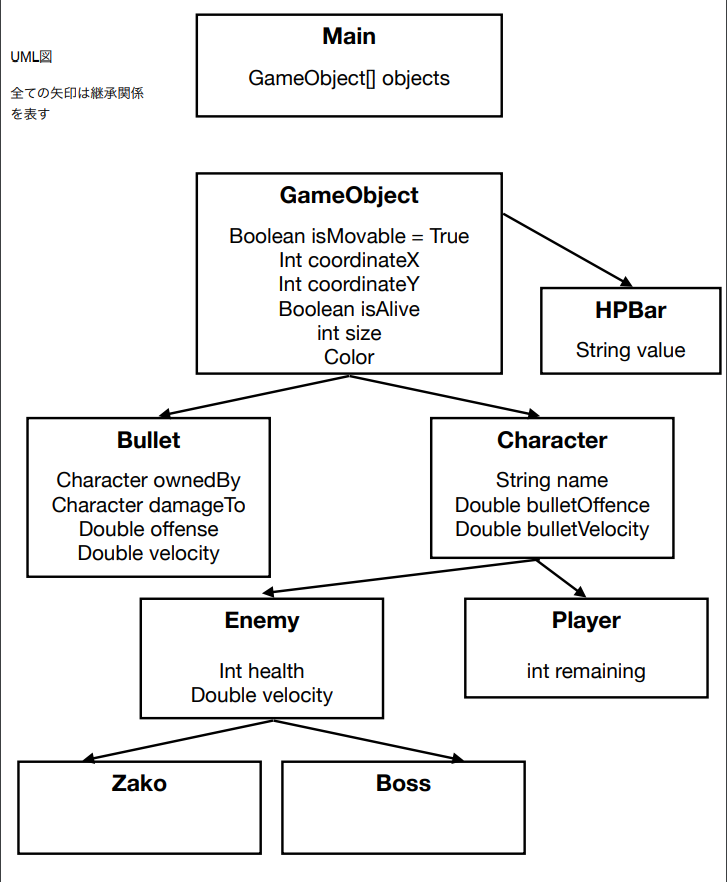
\includegraphics[width=150mm]{figures/class.png}
  \caption{クラス設計図}
  \label{fig:model}
\end{figure}

\section{実行結果}
図\ref{fig:a}の画面からスタートする.図\ref{fig:b}のように球が発射されダメージを与えた分HPバーが減少する.図\ref{fig:c}はすべての敵を倒した状態である.
\begin{figure}[H]
\centering
\begin{minipage}[b]{0.32\columnwidth}
    \centering
    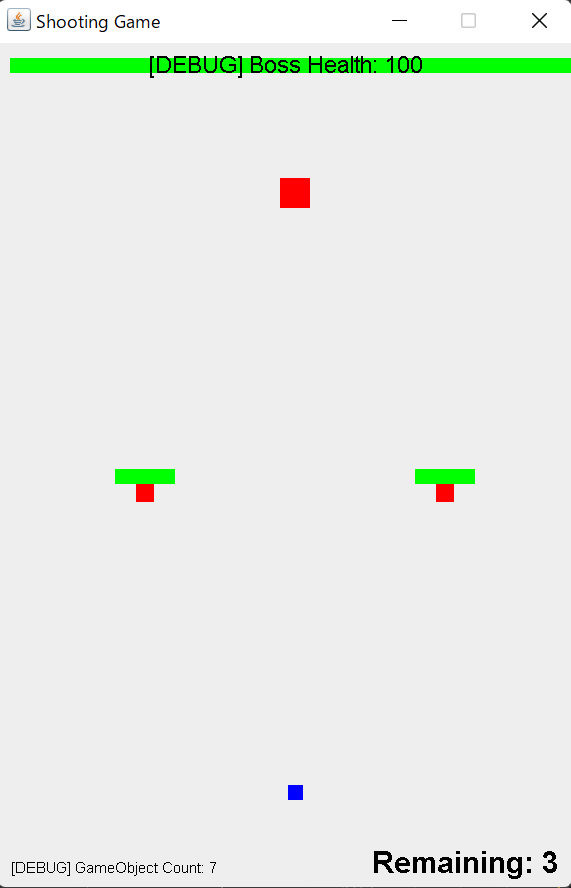
\includegraphics[width=0.7\columnwidth]{figures/result1.png}
    \caption{実行画面1}
    \label{fig:a}
\end{minipage}
\begin{minipage}[b]{0.32\columnwidth}
    \centering
    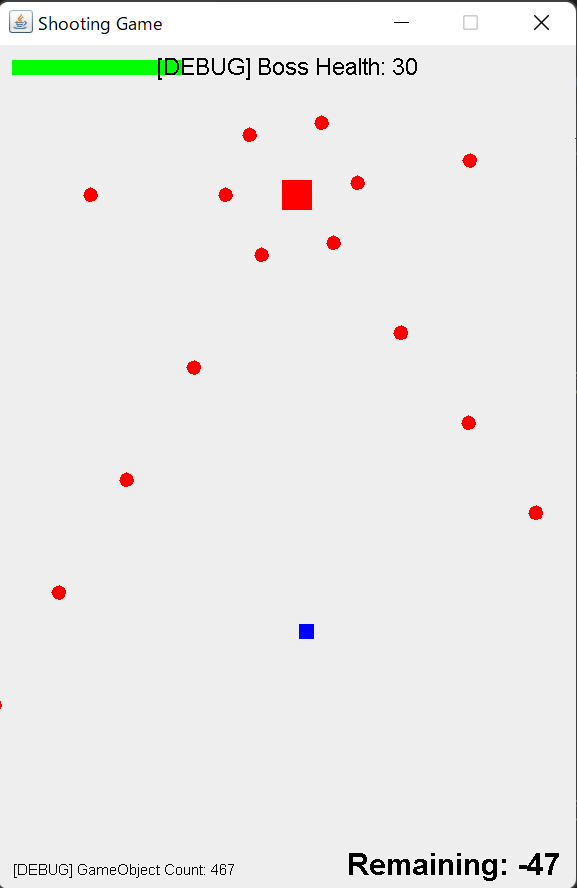
\includegraphics[width=0.7\columnwidth]{figures/result3.png}
    \caption{実行画面2}
    \label{fig:b}
\end{minipage}
\begin{minipage}[b]{0.32\columnwidth}
    \centering
    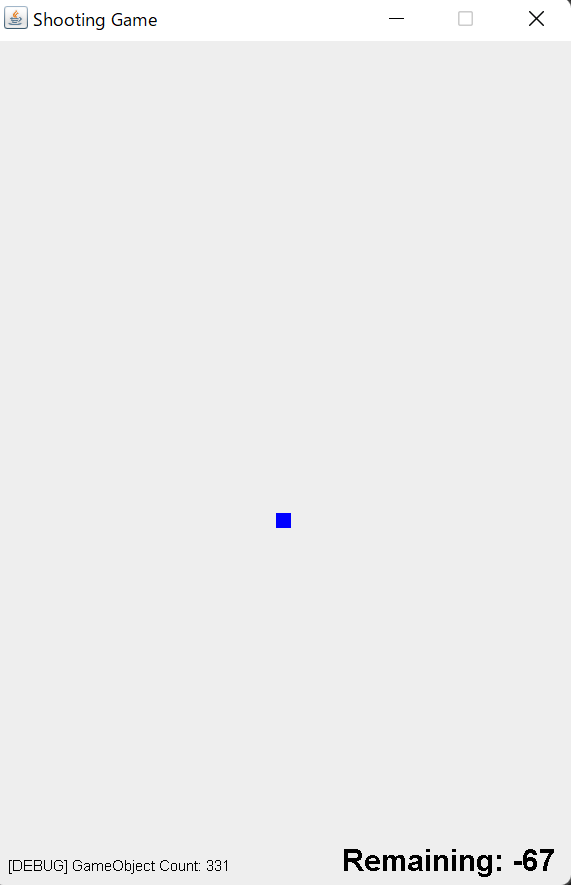
\includegraphics[width=0.7\columnwidth]{figures/result4.png}
    \caption{実行画面3}
    \label{fig:c}
\end{minipage}
\end{figure}

\section{クラス設計に対する考察}
今回のクラス設計では保守性,可読性ともに高まったといえる.GameObjectクラスから,Characterクラス,HPBarクラス,Bulletクラスに分けたことでそれぞれの管理がしやすくなりコードの可読性も高まった.また,新たに中ボスなどをつくる際もEnemyクラスがあることでコードの追加が容易であると考えられるため,保守性・拡張性も高いと言える.

\section{ソースコード}
コードをGitHubに掲載した.URLを以下に示す.

\url{https://github.com/Piertotum-Locomotor/kthr_shooting}

\newpage

\section{担当箇所}
筆者らの担当した箇所を以下の表\ref{contribution}に示す.

\begin{table}[hbtp]
  \caption{執筆者らの担当箇所}
  \label{contribution}
  \centering
  \begin{tabular}{|c|c|}
    \hline
    内容 & 名前 \\
    \hline\hline
    レポート本文作成 & 千本木,本江 \\
    \hline
    クラス設計草案 &  千本木,池田\\
    \hline
    クラス設計清書 &  千本木\\
    \hline
    AIによる雛形作成 & 池田 \\
    \hline
    プログラミング & 千本木,本江,池田 \\
    \hline
    \LaTeX 化 & 本江\\
    \hline
  \end{tabular}
\end{table}


\end{document}
